
\begin{question}
Solve the system of equations.

\[\begin{aligned}
2 x^{2} - 4 x + y &= -4 \\
16 x - y &= -24
\end{aligned}\]
\end{question}

\begin{solution}
There is no solution.

This system represents a parabola and a non-intersecting line.

\begin{figure}
\centering
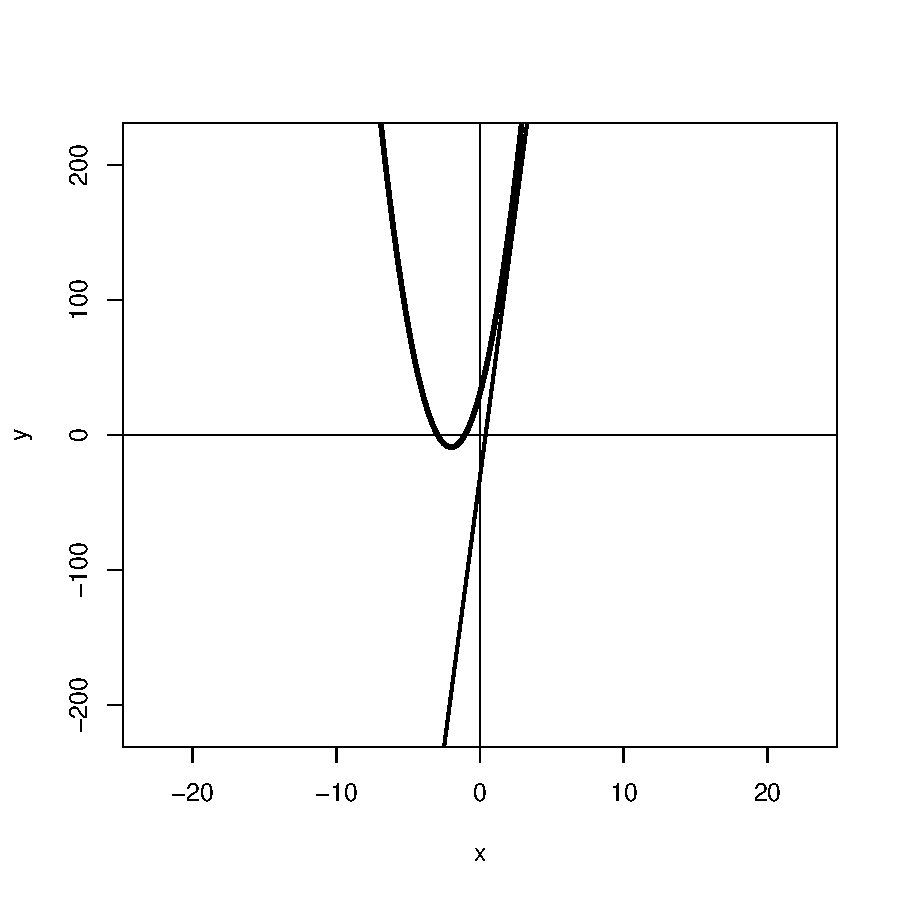
\includegraphics{unnamed-chunk-2-1-3.pdf}
\caption{plot of chunk unnamed-chunk-2}
\end{figure}
\end{solution}

